\Opensolutionfile{ans}[ans/ansCD2D1-5-G]

\begin{dang}{Phương trình tiếp tuyến của đồ thị hàm số}
\end{dang}
\paragraph{Các ví dụ}
\begin{vd}%Ví dụ 1.%[Lương Như Quỳnh, TLDH1]%[2D1Y5-6]
	Tiếp tuyến của đồ thị hàm số $y=x^3-2x+3$ tại điểm $M(1; 2)$ có hệ số góc bằng
	\choice
	{$3$}
	{$0$}
	{$2$}
	{\True $1$}
	\loigiai{
	$y'=3x^2-2$ nên hệ số góc của tiếp tuyến là $y'(1)=3\cdot 1-2 =1$.}
\end{vd}
\begin{vd}%Ví dụ 2.%[Lương Như Quỳnh, TLDH1]%[2D1Y5-6]
	Cho hàm số $y=x^3+2x^2+1$ có đồ thị là $(C)$. Phương trình tiếp tuyến của $(C)$ tại $M(1;4)$ là 
	\choice
	{$y=3x+1$}
	{\True $y=7x-3$}
	{$y=7x+2$}
	{$y=-x+5$}
	\loigiai{
		Ta có $y'=3x^2+4x\Rightarrow y'(1)=7$.\\
		Phương trình tiếp tuyến của $(C)$ tại $M(1;4)$ là $y=7(x-1)+4=7x-3$.}
\end{vd}
\begin{vd}%Ví dụ 3.%[Lương Như Quỳnh, TLDH1]%[2D1B5-6]
	Đường thẳng $y=m-1$ tiếp xúc với đồ thị $(C)\colon y=2x^4-4x^2+1$ tại hai điểm phân biệt. Tung độ của tiếp điểm là 
	\choice
	{$2$}
	{$1$}
	{$-2$}
	{\True $-1$}
	\loigiai{
		Xét hàm số $y=2x^4-4x^2+1$ trên $\mathbb{R}$.\\
		Ta có $y'=8x^3-16x$; $y'=0\Leftrightarrow 8x^3-8x=0\Leftrightarrow\hoac{&x=0\\&x=\pm 1.}$ \\
		Bảng biến thiên
\begin{center}

\begin{tikzpicture}
\tikzset{double style/.append style = {double distance=2pt}} 
\tkzTabInit[nocadre=false,lgt=1.2,espcl=2.5,deltacl=0.6] 
{$x$ /.6, $f’(x)$ /.6, $f(x)$/2}
{$-\infty$ , $-1$ , $0$ ,$ 1 $, $+\infty$}%
\tkzTabLine { , - , z , + , z , - , z , + , }
\tkzTabVar {+/$+\infty$,-/$ -1 $ ,+/$1$, -/$-1$ , +/$+\infty$}
\end{tikzpicture}
\end{center}
		Để đường thẳng $y=m-1$ tiếp xúc với đồ thị $(C)$ thì $ m-1=-1\Leftrightarrow m=0 $.\\
		Khi đó tung độ tiếp điểm $y=-1$.}
\end{vd}
\begin{vd}%Ví dụ 4.%[Lương Như Quỳnh, TLDH1]%[2D1B5-6]
	Cho hàm số $y=\dfrac{-x+1}{x+2}$ có đồ thị $(C)$. Gọi $d$ là tiếp tuyến của $(C)$ biết $d$ song song với đường thẳng $y=-3x-1$. Phương trình đường thẳng $d$ có dạng $y=ax+b$ với $a$, $b\in\mathbb{Z}$. Tính $S=a^3-b^2$. 
	\choice
	{\True $S=-196$}
	{$S=-52$}
	{$S=-2224$}
	{$S=-28$}
	\loigiai{
		Vì $d$ song song với đường thẳng $y=-3x-1$ nên hệ số góc tiếp tuyến là $$k=y'\left(x_0\right)=\dfrac{-3}{\left(x_0+2\right)^2}=-3\Leftrightarrow \left(x_0+2\right)^2=1\Leftrightarrow\hoac{&x_0=-1 \,\text{(loại)}\\&x_0=-3 \,\text{(nhận)}.}$$ 
		Với $x_0=-3$ ta có phương trình tiếp tuyến là $y=-3(x+3)-4=-3x-13$ suy ra $a=-3$, $b=-13$. \\
		Vậy $S=a^3-b^2=-196$.}
\end{vd}
\begin{vd}%Ví dụ 5.%[Lương Như Quỳnh, TLDH1]%[2D1K5-6]
	Cho hàm số $ y=\dfrac{2x+1}{x-1} $ có đồ thị $ (C) $. Tiếp tuyến của đồ thị $ (C) $ tại điểm thuộc đồ thị $ (C) $ có hoành độ $ x_0=\sqrt[3]{4} $ cắt hai đường tiệm cận của đồ thị hàm số tại hai điểm $ A $, $ B $. Tính diện tích tam giác $ IAB $ với $ I $ là giao điểm của hai đường tiệm cận của đồ thị hàm số $ (C) $. 
	\choice
	{\True $ S=6 $}
	{$ S=6\sqrt[3]{2} $}
	{$ S=3 $}
	{$ S=12 $}
	\loigiai{
		Giao điểm của hai đường tiệm cận là $ I(1;2) $.\\
		Phương trình tiếp tuyến của $ (C) $ tại điểm $ x=x_0 $ là $ y=-\dfrac{3}{\left(x_0-1\right)^2}\left(x-x_0\right) +\dfrac{2x_0+1}{x_0-1}$.\\
		Gọi $ A $ là giao điểm của tiếp tuyến với tiệm cận đứng $ \Rightarrow A \left(1;\dfrac{2x_0+4}{x_0-1} \right)$.\\
		Gọi $ B $ là giao điểm của tiếp tuyến với tiệm cận ngang $ \Rightarrow B \left(2x_0-1;2 \right)$.\\
		Diện tích tam giác $ IAB $ là $ S=\dfrac{1}{2}IA \cdot IB = \dfrac{1}{2} \sqrt{\left(\dfrac{6}{x_0-1} \right)^2}\cdot \sqrt{\left( 2x_0-2 \right)^2}=6 $.
		}
\end{vd}
\paragraph{Câu hỏi trắc nghiệm}
\begin{ex}%Câu 1.%[Lương Như Quỳnh, TLDH1]%[2D1B5-6]
	Viết phương trình tiếp tuyến của đồ thị hàm số $y=\dfrac{x-1}{x+1}$ tại điểm $M(0;-1)$. 
	\choice
	{$y=x-1$}
	{$y=-x-1$}
	{\True $y=2x-1$}
	{$y=3x-1$}
	\loigiai{
		Ta có $y'=\dfrac{2}{(x+1)^2}\Rightarrow y'(0)=2$ nên phương trình tiếp tuyến là $y=2x-1$.}
\end{ex}
\begin{ex}%Câu 2.%[Lương Như Quỳnh, TLDH1]%[2D1B5-6]
	Phương trình tiếp tuyến của đồ thị hàm số $y=x^3-3x^2+2$ tại điểm có hoành độ bằng $-1$ là
	\choice
	{$y=-3x-5$}
	{$y=-9x+7$}
	{\True $y=9x+7$}
	{$y=9x-11$}
	\loigiai{
		Ta có $y'=3x^2-6x$.\\
		Gọi $\Delta$ là tiếp tuyến và $M \left(x_0;y_0\right)$ là tiếp điểm.\\
		Ta có $x_0=-1\Rightarrow y_0=-2$; $y'(-1)=9$.\\
		Vậy $\Delta\colon y=9x+7$.}
\end{ex}
\begin{ex}%Câu 3.%[Lương Như Quỳnh, TLDH1]%[2D1B5-6]
	Gọi $\Delta$ là tiếp tuyến tại điểm cực tiểu của đồ thị hàm số $y=\dfrac{x^3}{3}-2x^2+3x-5$. Chọn khẳng định đúng. 
	\choice
	{\True $\Delta$ song song với trục hoành}
	{$\Delta$ có hệ số góc âm}
	{$\Delta$ song song với trục tung}
	{$\Delta$ có hệ số góc dương}
	\loigiai{
		Hàm số đã cho là hàm đa thức nên tại điểm cực tiểu thì $y'=0$ \\
		Do đó tiếp tuyến tại điểm cực tiểu của đồ thị hàm số có hệ số góc bằng 0.}
\end{ex}
\begin{ex}%Câu 4.%[Lương Như Quỳnh, TLDH1]%[2D1B5-6]
	Cho hàm số $f(x)=x^3-3x^2+2x+2018$. Tiếp tuyến của đồ thị hàm số tại điểm $M(0;1)$ có hệ số góc là 
	\choice
	{$1$}
	{\True $2$}
	{$0$}
	{$-1$}
	\loigiai{
		Ta có $f'(x)=3x^2-6x+2$.\\
		Tiếp tuyến của đồ thị hàm số tại điểm $M(0;1)$ có hệ số góc là $k=f'(0)=2$.}
\end{ex}
\begin{ex}%Câu 5.%[Lương Như Quỳnh, TLDH1]%[2D1Y5-6]
	Viết phương trình tiếp tuyến của đồ thị hàm số $y=f(x)=x^2$ tại điểm có hoành độ bằng $2$. 
	\choice
	{$y=2x$}
	{$y=(4\ln 2)x-8\ln 2+4$}
	{$y=4(1+\ln 2)x-8\ln 2-4$}
	{\True $y=4x-4$}
	\loigiai{
		Gọi $\left(x_0;y_0 \right)$ là tiếp điểm. Ta có $x_0=2\Rightarrow y_0=4$. Mà $y'=2x\Rightarrow y'(2)=4$.\\
		Vậy phương trình tiếp tuyến cần tìm là $y=4(x-2)+4$ hay $y=4x-4$.}
\end{ex}
\begin{ex}%Câu 6.%[Lương Như Quỳnh, TLDH1]%[2D1B5-6]
	Viết phương trình tiếp tuyến của hàm số $y=\dfrac{x-1}{x+2}$ tại điểm có hoành độ $x_0=-3$. 
	\choice
	{\True $y=3x+13$}
	{$y=-3x-5$}
	{$y=-3x+13$}
	{$y=3x+15$}
	\loigiai{
		Ta có $x_0=-3\Rightarrow y_0=\dfrac{x_0-1}{x_0+2}=\dfrac{-3-1}{-3+2}=4$.\\
		Và $f'(x_0)=\dfrac{3}{(x_0+2)^2}=\dfrac{3}{(-3+2)^2}=3$.\\
		Phương trình tiếp tuyến tại điểm có $x_0=-3$ là 
		\begin{eqnarray*}
		&&y=f'\left(x_0\right) \left(x-x_0\right)+y_0\\
		&\Leftrightarrow& y=3(x+3)+4\\
		&\Leftrightarrow& y=3x+13.
		\end{eqnarray*}		
		}
\end{ex}
\begin{ex}%Câu 7.%[Lương Như Quỳnh, TLDH1]%[2D1B5-6]
	Cho hàm số $y=\dfrac{2x+1}{2x-1}$ có đồ thị $(C)$. Hệ số góc của tiếp tuyến với $(C)$ tại điểm có hoành độ bằng $1$ là
	\choice
	{\True $-4$}
	{$4$}
	{$0$}
	{$1$}
	\loigiai{
		Ta có $y'=\dfrac{-4}{(2x-1)^2}$.\\
		Hệ số góc của tiếp tuyến là $k=y'(1)=-4$.}
\end{ex}
\begin{ex}%Câu 8.%[Lương Như Quỳnh, TLDH1]%[2D1Y5-6]
	Hệ số góc của tiếp tuyến với đồ thị hàm số $f(x)=-x^3$ tại điểm $M(-2; 8)$ là
	\choice
	{$-192$}
	{\True $-12$}
	{$192$}
	{$12$}
	\loigiai{
		Ta có $y'=-3x^2$ nên hệ số góc của tiếp tuyến là $y'(-2)=-12$.}
\end{ex}
\begin{ex}%Câu 9.%[Lương Như Quỳnh, TLDH1]%[2D1B5-6]
	Đường thẳng $(\Delta)$ là tiếp tuyến của đồ thị hàm số $y=x^4+3x^2-2$ tại điểm có hoành độ bằng $1$. Hệ số góc của đường thẳng $(\Delta)$ bằng bao nhiêu?
	\choice
	{$5$}
	{\True $10$}
	{$6$}
	{$-12$}
	\loigiai{
		Tập xác định: $ \mathscr{D} = \mathbb{R}$.\\
		Ta có $ y'=4x^3+6x$.\\
		Hệ số góc của tiếp tuyến tại điểm có hoành độ bằng $1$ là $y'(1)=10$.}
%<MyLT>
\end{ex}
\begin{ex}%Câu 10.%[Lương Như Quỳnh, TLDH1]%[2D1B5-6]
	Đường thẳng nào sau đây là tiếp tuyến kẻ từ điểm $M(2;-1)$ đến đồ thị hàm số $y=\dfrac{x^2}{4}-x+1$? 
	\choice
	{$y=-2x+3$}
	{$y=-1$}
	{\True $y=x-3$}
	{$y=3x-7$}
	\loigiai{
		Gọi $M \left(x_0;y_0\right)$ là tiếp điểm của tiếp tuyến cần tìm, khi đó phương trình tiếp tuyến là
		$$y=\left(\dfrac{x_0}{2}-1\right)\left(x-x_0\right)+\dfrac{x_0^2}{4}-x_0+1.$$
		Do tiếp tuyến kẻ từ điểm $M(2;-1)$ nên
		\begin{eqnarray*}
		&&-1=\left(\dfrac{x_0}{2}-1\right)(2-x_0)+\dfrac{x_0^2}{4}-x_0+1\\
		&\Leftrightarrow& -\dfrac{x_0^2}{4}+x_0=0\\
		&\Leftrightarrow& \hoac{&x_0=0\\&x_0=4.}
		\end{eqnarray*}
		Tiếp tuyến tại $M(0;1)$ là $y=-x+1$.\\
		Tiếp tuyến tại $M(4;1)$ là $y=x-3$.}
\end{ex}
\begin{ex}%Câu 11.%[Lương Như Quỳnh, TLDH1]%[2D1B5-6]
	Cho hàm số $y=\dfrac{x-1}{x+1}$ có đồ thị là $(C)$. Tiếp tuyến của $(C)$ tại giao điểm của đồ thị với trục tung có phương trình là 
	\choice
	{$x+2y+1=0$}
	{$2x+y+1=0$}
	{$x-2y-1=0$}
	{\True $2x-y-1=0$}
	\loigiai{
Xét hàm số $y=\dfrac{x-1}{x+1}$ có tập xác định $\mathscr{D}=\mathbb{R}\setminus\{-1\}$.\\
Ta có $y'=\dfrac{2}{(x-1)^2}$. \\
Giao điểm của đồ thị hàm số với tục tung có tọa độ là $A(0;-1)$ nên phương trình tiếp tuyến của đồ thị hàm số tại $A(0;-1)$ là 
\begin{eqnarray*}
&& y=f'(0)(x-0)-1\\
&\Leftrightarrow& y=2x-1\\
&\Leftrightarrow& 2x-y-1=0.
\end{eqnarray*}
}
\end{ex}
\begin{ex}%Câu 12.%[Lương Như Quỳnh, TLDH1]%[2D1B5-6]
	Tiếp tuyến của đồ thị hàm số $y=\dfrac{3x-1}{x-3}$ song song với đường thẳng $y=-2x+1$. 
	\choice
	{$0$}
	{$2$}
	{$3$}
	{\True $1$}
	\loigiai{
		$y=\dfrac{3x-1}{x-3}\Rightarrow y'=\dfrac{-8}{(x-3)^2}$.\\
		Ta có $y'=-2\Leftrightarrow\dfrac{-8}{(x-3)^2}=-2\Leftrightarrow\hoac{&x=5\\&x=1.}$\\
		Phương trình tiếp tuyến của đồ thị tại $M(5;7)\colon y=-2(x-5)+7=-2x+17$.\\
		Phương trình tiếp tuyến của đồ thị tại $M(1;-1)\colon y=-2(x-1)-1=-2x+1 \,\text{(loại)}$.}
\end{ex}
\begin{ex}%Câu 13.%[Lương Như Quỳnh, TLDH1]%[2D1B5-6]
	Phương trình tiếp tuyến của đường cong $y=x^3+3x^2-2$ tại điểm có hoành độ $x_0=1$ là 
	\choice
	{\True $y=9x-7$}
	{$y=9x+7$}
	{$y=-9x-7$}
	{$y=-9x+7$}
	\loigiai{
		Ta có $y'=3x^2+6x$; $y'\left(x_0\right)=y'(1)=9$.\\
		$x_0=1\Rightarrow y_0=2$.\\
		Phương trình tiếp tuyến cần tìm là $y=y'\left(x_0\right)\cdot \left(x-x_0\right)+y_0\Leftrightarrow y=9x-7$.}
\end{ex}
% \begin{ex}%Câu 14.%[Lương Như Quỳnh, TLDH1]%[2D1K5-6]
% 	Họ parabol $\left(P_m \right)\colon y=mx^2-2(m-3)x+m-2$ $(m\neq 0)$ luôn tiếp xúc với đường thẳng $d$ cố định khi $m$ thay đổi. Đường thẳng $d$ đó đi qua điểm nào dưới đây?
% 	\choice
% 	{$(0;-2)$}
% 	{\True $(0;2)$}
% 	{$(1; 8)$}
% 	{$(1;-8)$}
% 	\loigiai{
% 		Ta có $(P_m)\colon y=mx^2-2(m-3)x+m-2\Rightarrow(P_m)\colon y=m(x-1)^2+6x-2$.\\
% 		Do đó $(P_m)$ luôn tiếp xúc với đường thẳng $d\colon y=-6x+2$ với mọi $m\neq 0\Rightarrow(0; 2)\in d$.}
% \end{ex}
\begin{ex}%Câu 15.%[Lương Như Quỳnh, TLDH1]%[2D1K5-6]
	Số tiếp tuyến của đồ thị hàm số $f(x)=x^4-2x^2+10$ song song với trục hoành là
	\choice
	{$1$}
	{$0$}
	{$3$}
	{\True $2$}
	\loigiai{
		Ta có $f'(x)=4x^3-4x$.\\
		Vì tiếp tuyến song song với trục hoành nên $f'(x)=4x^3-4x=0\Leftrightarrow\hoac{&x=0\\&x=\pm 1.}$ \\
		Trường hợp 1: $x=0\Rightarrow$ Tiếp điểm $M_1(0;10)\Rightarrow$ Tiếp tuyến $d_1\colon y=10$ (thỏa mãn $d_1\parallel Ox$).\\
		Trường hợp 2: $x=1\Rightarrow$ Tiếp điểm $M_2(1;9)\Rightarrow$ Tiếp tuyến $d_2\colon y=9$ (thỏa mãn $d_2\parallel Ox$).\\
		Trường hợp 3: $x=-1\Rightarrow$ Tiếp điểm $M_3(-1;9)\Rightarrow$ Tiếp tuyến $d_3\colon y=9$ (thỏa mãn $d_3\parallel Ox$) và $d_3\equiv d_2$.\\
		Từ đó suy ra đồ thị hàm số $f(x)=x^4-2x^2+10$ có $2$ tiếp tuyến song song với trục hoành.}
\end{ex}
\begin{ex}%Câu 16.%[Lương Như Quỳnh, TLDH1]%[2D1K5-6]
\immini{
	Cho hàm số $y=f(x)$ có đồ thị là đường cong $(C)$. Biết đồ thị của hàm số $y=f'(x)$ như hình vẽ và tiếp tuyến với $(C)$ tại điểm $M$ có hoành độ bằng $1$ cắt đồ thị $(C)$ tại hai điểm khác nữa là $A$ và $B$ lần lượt có hoành độ $a$, $b$. Mệnh đề nào dưới đây đúng?
	\choice
	{$a,b >-1$}
	{$|a-b|\leq 4$}
	{\True $a^2+b^2>10$}
	{$a,b<3$}}
	{
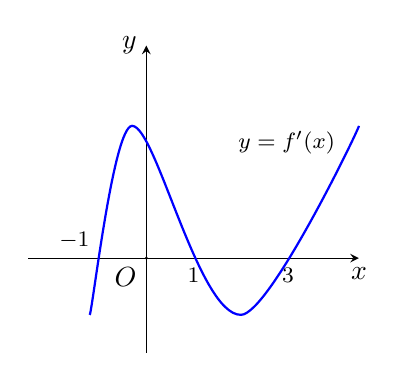
\begin{tikzpicture}[thin,scale=.6]
\draw[-stealth] (-2.5,0)--(4.5,0) node[below]{$x$};
\draw[-stealth] (0,-2)--(0,4.5) node[left]{$y$};
\draw[fill=white] (0,0)coordinate (O) circle(.5pt)node[below left]{$O$};
\draw(-1,0) node[above left]{\footnotesize $-1$};
\foreach \x in{1,3}\draw(\x,0) node[below]{\footnotesize $\x$};
\draw(4.2,2) node[above left]{\footnotesize $y=f'(x)$};
\coordinate (A) at (-1.2,-1.2);
\coordinate (B) at (-.3,2.8);
\coordinate (C) at (2,-1.2);
\coordinate (D) at (4.5,2.8);
\draw[thick,blue]
(A) .. controls +(0:.05) and +(-180:.4) ..
(B) .. controls +(0:.5) and +(180:.9) ..
(C) .. controls +(0:.6) and +(-80:.05)..
(D);
\end{tikzpicture}		
	}
	\loigiai{
		Ta có bảng biến thiên của hàm số:
	\begin{center}
\begin{tikzpicture}[yscale=.5]
\draw 
(-.5,.5) rectangle +(10,-5)
(-.5,-.5)--+(0:10) (-.5,-1.5)--+(0:10) (.5,.5)--+(-90:5);
\path[blue] 
(0,0) node{$x$}
(0,-1) node{$y'$}
(0,-3) node{$y$}

(1,0) node{$-\infty$}
(3,0) node{$-1$}
(5,0) node{$1$}
(7,0) node{$3$}
(9,0) node{$+\infty$}

(1,-2) node(A){$+\infty$}
(3,-4) node(B){$\text{CT}$}
(5,-2) node(C){$\text{CĐ}$}
(7,-4) node(D){$\text{CT}$}
(9,-2) node(E){$+\infty$}

(2,-1) node{$-$}
(4,-1) node{$+$}
(6,-1) node{$-$}
(8,-1) node{$+$}
(3,-1) node{$0$}
(5,-1) node{$0$}
(7,-1) node{$0$};

\draw[->,magenta] (A)--(B);
\draw[->,magenta] (B)--(C);
\draw[->,magenta] (C)--(D);
\draw[->,magenta] (D)--(E);
\end{tikzpicture}
	\end{center}
Tiếp tuyến của đồ thị tại $M$ có hoành độ bằng $1$ là đường thẳng song song với trục $Ox$ cắt đồ thị hàm số tại ba điểm $A$, $B$ và cực đại biểu thị như hình
	\begin{center}
\begin{tikzpicture}[yscale=.5]
\draw 
(-.5,.5) rectangle +(10,-5)
(-.5,-.5)--+(0:10) (-.5,-1.5)--+(0:10) (.5,.5)--+(-90:5);
\path[blue] 
(0,0) node{$x$}
(0,-1) node{$y'$}
(0,-3) node{$y$}

(1,0) node{$-\infty$}
(2,0) node{$a$}
(3,0) node{$-1$}
(5,0) node{$1$}
(7,0) node{$3$}
(8,0) node{$b$}
(9,0) node{$+\infty$}

(1,-2) node(A){$+\infty$}
(3,-4) node(B){$\text{CT}$}
(5,-2) node(C){$\text{CĐ}$}
(7,-4) node(D){$\text{CT}$}
(9,-2) node(E){$+\infty$}

(2,-1) node{$-$}
(4,-1) node{$+$}
(6,-1) node{$-$}
(8,-1) node{$+$}
(3,-1) node{$0$}
(5,-1) node{$0$}
(7,-1) node{$0$};

\draw[->,magenta] (A)--(B);
\draw[->,magenta] (B)--(C);
\draw[->,magenta] (C)--(D);
\draw[->,magenta] (D)--(E);
\end{tikzpicture}
	\end{center}
		Với $a$, $b$ lần lượt là các hoành độ giao điểm của hai điểm $A$, $B$.\\
		Vậy $a^2>1$, $b^2>3^3\Rightarrow a^2+b^2>10$.}
\end{ex}
\begin{ex}%Câu 17.%[Lương Như Quỳnh, TLDH1]%[2D1K5-6]
	Cho hàm số $y=\dfrac{x-3}{-x+1}$ có đồ thị $(C)$ và điểm $A(a; 1)$. Gọi $S$ là tập tất cả các giá trị thực của $a$ để có đúng một tiếp tuyến của $(C)$ đi qua $A$. Tổng giá trị tất cả các phần tử của $S$ bằng
	\choice
	{$\dfrac{4}{3}$}
	{\True $3$}
	{$\dfrac{7}{2}$}
	{$2$}
	\loigiai{
		$y=\dfrac{x-3}{-x+1}\Rightarrow y'=\dfrac{-2}{(1-x)^2} (C)$.\\
		Gọi $d$ là đường thẳng qua $A(a; 1)$ có hệ số góc $k$.\\
		Khi đó $d\colon y=kx-ka+1$.\\
		Xét hệ phương trình 
\begin{eqnarray*}		
		&&\heva{&\dfrac{x-3}{-x+1}=k(x-a)+1\\&k=\dfrac{-2}{(1-x)^2}} \\
		&\Rightarrow& \dfrac{x-3}{1-x}=-\dfrac{2}{(1-x)^2}(x-a)+1\quad(x\neq 1)\\
		&\Leftrightarrow& x^2-4x+a+2=0 \quad(*).
		\end{eqnarray*}
		Ta xét hai trường hợp:
		\begin{itemize}
		\item Trường hợp 1: Phương trình có nghiệm kép khác $ 1 $. Khi đó
		 $$\heva{&4-a-2=0\\&1-4+a+2\neq 0}\Leftrightarrow\heva{&a=2\\&a\neq 1}\Rightarrow a=2.$$
		\item Trường hợp 2: Phương trình có hai nghiệm phân biệt, trong đó có một nghiệm bằng $ 1 $.\\
		Thế $x=1$ vào ta được $a=1$.\\
		Với $a=1$: phương trình trở thành $x^2-4x+3=0\Leftrightarrow \hoac{&x=1\\& x=3.}$\\
		Do đó nhận $a=1$.
		\end{itemize}
		Vậy $S=\{1;2\}$. Suy ra tổng các phần tử của $ S $ bằng $ 3 $.}
\end{ex}
\begin{ex}%Câu 18.%[Lương Như Quỳnh, TLDH1]%[2D1K5-6]
	Cho đồ thị hàm số $(C)\colon y=f(x)=2x^3-3x^2+5$. Từ điểm $A\left(\dfrac{19}{12};4\right)$ có thể kẻ được bao nhiêu tiếp tuyến tới $(C)$?
	\choice
	{$1$}
	{$2$}
	{$4$}
	{\True $3$}
	\loigiai{
		Gọi $M\left(x_0;2x_0^3-3x_0^2+5\right)$ là tiếp điểm của tiếp tuyến đi qua $A\left(\dfrac{19}{12};4\right)$.\\
		Phương trình tiếp tuyến tại $M$ là 
		\begin{eqnarray*}
		y&=&f'\left(x_0\right) \left(x-x_0\right)+y_0\\
		&=&\left(6x_0^2-6x_0\right)(x-x_0)+2x_0^3-3x_0^2+5 \quad(d).
		\end{eqnarray*}
		Do $A\in d$ nên
		\begin{eqnarray*}
		&&  4=\left(6x_0^2-6x_0\right)\left(\dfrac{19}{12}-x_0\right)+2x_0^3-3x_0^2+5\\
		&\Leftrightarrow&-4x_0^3+\dfrac{25}{2}x_0^2-\dfrac{19}{2}x_0+1=0 \\
		&\Leftrightarrow& \hoac{&x=\dfrac{1}{8}\\&x=1\\&x=2.}
		 \end{eqnarray*}
		Vậy có $3$ tiếp tuyến kẻ từ $A\left(\dfrac{19}{12};4\right)$.}
\end{ex}
\begin{ex}%Câu 19.%[Lương Như Quỳnh, TLDH1]%[2D1K5-6]
	Gọi $M(a;b)$ là điểm trên đồ thị $(C)$ của hàm số $y=\dfrac{1}{x-1}$ sao cho tiếp tuyến $(C)$ tại $M$ cùng với các trục tọa độ tạo thành tam giác có diện tích bằng $2$. Khi đó
	\choice
	{\True $ab=-3$}
	{$ab=-1$}
	{$ab=4$}
	{$ab=2$}
	\loigiai{
		Tiếp tuyến tại $M(a;b)$ là 
		\begin{eqnarray*}
		&&y=\dfrac{-1}{(a-1)^2}(x-a)+b\\
		&\Leftrightarrow& y=\dfrac{-1}{(a-1)^2}\cdot x+\dfrac{a}{(a-1)^2}+b.
		\end{eqnarray*}
		Và $b=\dfrac{1}{a-1}$.\\
		Giao của tiếp tuyến với trục hoành $A\left(a+b(a-1)^2;0\right)$ hay $A(2a-1;0)$.\\
		Giao tiếp tuyến với trục tung $B\left(0;\dfrac{a}{(a-1)^2}+b\right)$ hay $B\left(0;\dfrac{2a-1}{(a-1)^2}\right)$.\\
		Theo giả thiết 
		\begin{eqnarray*}
		&&S_{OAB}=2\Rightarrow OA\cdot OB=4\\
		&\Leftrightarrow& (2a-1)^2=4(a-1)^2\\
		&\Leftrightarrow& a=\dfrac{3}{4}.
		\end{eqnarray*}
		Suy ra $ b=-4 $. Vậy $ ab=-3 $.}
\end{ex}
\begin{ex}%Câu 20%[Lương Như Quỳnh, TLDH1]%[2D1K5-6]
Cho hàm số $y=\dfrac{x+2}{2x+3}$ $(C)$. Phương trình tiếp tuyến của đồ thị hàm số biết tiếp tuyến đó cắt trục hoành và trục tung lần lượt tại hai điểm phân biệt $ A $, $ B $ và tam giác $ OAB $ cân tại $ O $ là 
	\choice
	{$y=-x+1$}
	{\True $y=-x-2$}
	{$y=-x+2$}
	{$y=-x$}
	\loigiai{
Ta có $ y'=\dfrac{-1}{(2x+3)^2} $.\\
		Phương trình tiếp tuyến tại $M\left(a;\dfrac{a+2}{2a+3}\right)$ là 
$$y=\dfrac{-1}{(2a+3)^2}(x-a)+\dfrac{a+2}{2a+3}.$$
		Giao của tiếp tuyến với trục hoành $A\left(2a^2+8a+6;0\right)$.\\
		Giao tiếp tuyến với trục tung $B\left(0;\dfrac{2a^2+8a+6}{(2a+3)^2}\right)$.\\
		Để tam giác $ OAB $ cân tại $ O $ thì $ OA=OB $, khi đó
		\begin{eqnarray*}
		&&\left| { 2a^2+8a+6 } \right|=\dfrac{\left| { 2a^2+8a+6 } \right|}{(2a+3)^2}\\
		&\Rightarrow& (2a+3)^2=1\\
		&\Leftrightarrow& \hoac{&2a+3=1\\&2a+3=-1}\\
		&\Leftrightarrow& \hoac{&a=-1\\&a=-2.}
		\end{eqnarray*}
Với $ a=-1 $: Phương trình tiếp tuyến là $ y=-x$ (loại).\\
Với $ a=-2 $: Phương trình tiếp tuyến là $ y=-x-2 $.	
		}
\end{ex}
\begin{ex}%Câu 21%[Lương Như Quỳnh, TLDH1]%[2D1K5-6]
	Gọi $M$, $N$ là hai điểm di động trên đồ thị $(C)$ của hàm số $y=-x^3+3x^2-x+4$ sao cho tiếp tuyến của $(C)$ tại $M$ và $N$ luôn song song với nhau. Khi đó đường thẳng $MN$ luôn đi qua điểm cố định nào dưới đây?
	\choice
	{$(1;-5)$}
	{$(-1;-5)$}
	{$(-1;5)$}
	{\True $(1;5)$}
	\loigiai{
		Gọi $M(x_1; y_1)$, $N(x_2; y_2)\in(C)$. Do tiếp tuyến tại $M$, $N$ song song nhau ta có
		$$f'(x_1)=f'(x_2)\Rightarrow-3x_1^2+6x_1-1=-3x_2^2+6x_2-1\Leftrightarrow x_1+x_2=2.$$
		Đường thẳng $MN \colon$
\begin{eqnarray*}		
		 &&(y_2-y_1)(x-x_1)+(x_1-x_2)(y-y_1)=0 \\
		&\Leftrightarrow&\left[-x_2^3+3x_2^2-x_2+4-\left(-x_1^3+3x_1^2-x_1+4\right)\right](x-x_1)+(x_1-x_2)\left[y-\left(-x_1^3+3x_1^2-x_1+4\right)\right]=0\\
		&\Leftrightarrow& \left[x_1^2+x_1x_2+x_2^2-3(x_1+x_2)+1\right](x-x_1)+y-\left(-x_1^3+3x_1^2-x_1+4\right)=0 \\
		&\Leftrightarrow& \left[(x_1+x_2)^2-x_1x_2-3(x_1+x_2)+1\right](x-x_1)+y-\left(-x_1^3+3x_1^2-x_1+4\right)=0  \\
		&\Leftrightarrow& (-1-x_1x_2)(x-x_1)+y-\left(-x_1^3+3x_1^2-x_1+4\right)=0 \\
		&\Leftrightarrow& \left[-1-x_1(2-x_1)\right](x-x_1)+y-\left(-x_1^3+3x_1^2-x_1+4\right)=0 \\
		&\Leftrightarrow& \left(x_1^2-2x_1-1\right)x+y-x_1^2+2x_1-4=0  \\
		&\Leftrightarrow& (x-1)x_1^2+2(1-x)x_1+y-x-4=0 \quad(*).
		\end{eqnarray*}
	$ (*) $ đúng với mọi $x_1\Leftrightarrow\heva{&x-1=0\\&1-x=0\\&y-x-4=0}\Leftrightarrow\heva{&x=1\\&y=5.}$ \\
		Cách 2: Tiếp tuyến của $(C)$ tại $M$ và $N$ luôn song song với nhau nên đường thẳng $MN$ luôn đi qua điểm uốn của đồ thị.\\
		Ta có $y=-x^3+3x^2-x+4\Rightarrow y'=-3x^2+6x-1\Rightarrow y''=-6x+6=0\Rightarrow x=1\Rightarrow y=5$.}
\end{ex}
% \begin{ex}%Câu 22%[Lương Như Quỳnh, TLDH1]%[2D1K5-6]
% 	Cho hàm số $y=x^3-3x+2$ có đồ thị $(C)$. Hỏi có bao nhiêu điểm trên đường thẳng $d\colon y=9x-14$ sao cho từ đó kẻ được hai tiếp tuyến với $(C)$?
% 	\choice
% 	{\True $3$ điểm}
% 	{$4$ điểm}
% 	{$2$ điểm}
% 	{$1$ điểm}
% 	\loigiai{
% 		Ta có $y=x^3-3x+2\Rightarrow y'=3x^2-3$.\\
% 		Gọi $x_0$ là hoành độ tiếp điểm, phương trình tiếp tuyến có dạng
% 		$$y=\left(3x_0^2-3\right)(x-x_0)+x_0^3-3x_0+2.$$
% 		Gọi $M(m;9m-14)$ là điểm nằm trên đường thẳng $d\colon y=9x-14$.\\
% 		Tiếp tuyến đi qua điểm $M$ khi và chỉ khi
% 		\begin{eqnarray*}
% 		&& 9m-14=\left(3x_0^2-3\right)(m-x_0)+x_0^3-3x_0+2  \\
% 		&\Leftrightarrow& (x_0-2)\left[2x_0^2-(3m-4)x_0+8-6m\right]=0 \\
% 		&\Leftrightarrow& (x_0-2)\left[2x_0^2-(3m-4)x_0+8-6m\right]=0  \\
% 		&\Leftrightarrow& \hoac{&x_0=2\\&2x_0^2-(3m-4)x_0+8-6m=0=g(x_0)\quad(*).}
% 		\end{eqnarray*}
% 		Yêu cầu đề bài $\Leftrightarrow (*)$ có hai nghiệm phân biệt có một nghiệm bằng $2$ hoặc $(*)$ có nghiệm kép khác $2$. Khi đó
% 		\begin{eqnarray*}
% 		&&\heva{&\Delta>0\\&g(2)=0} \,\text{hoặc}\, \heva{&\Delta=0\\&g(2)\neq 0}\\
% 		&\Leftrightarrow& \hoac{&\heva{&9m^2+24m-48>0\\&-12m+24=0}\\&\heva{&9m^2+24m-48=0\\&-12m+24\neq 0}}\\
% 		&\Leftrightarrow& \hoac{&m=2\\&m=\dfrac{4}{3}\\&m=-4.}
% 		\end{eqnarray*}
% 		Vậy có $3$ điểm $M$ thỏa đề bài.}
% \end{ex}

% \begin{ex}%Câu 23%[Lương Như Quỳnh, TLDH1]%[2D1K5-6]
% 	Cho hàm số $y=\dfrac{1}{3}mx^3+(m-1)x^2+(4-3m)x+1$ có đồ thị là $(C_m)$, với $m$ là tham số. Tìm tất các các giá trị của $m$ để trên $(C_m)$ có duy nhất một điểm có hoành độ âm mà tiếp tuyến của $(C_m)$ tại điểm đó vuông góc với đường thẳng $d\colon x+2y=0$.	
% 	\choice
% 	{$M$}
% 	{$SD$}
% 	{\True $(ABM)$}
% 	{$(SCD)$}
% 	\loigiai{
% 		Ta có $y'=mx^2+2(m-1)x+4-3m$.\\
% 		$d\colon x+2y=0 \Leftrightarrow y=-\dfrac{1}{2}x$.\\
% 		Yêu cầu đề bài $ \Leftrightarrow mx^2+2(m-1)x+4-3m=2$ có đúng một nghiệm âm $ \Leftrightarrow mx^2+2(m-1)x+2-3m=0$ có đúng một nghiệm âm.\\
% 		Nếu $m=0$: $(1) \Leftrightarrow -2x+2=0 \Leftrightarrow x=$ không thỏa mãn.\\
% 		Nếu $m\ne 0$: có ba khả năng xảy ra.
% 		\begin{itemize}
% 		\item $(1)$ có hai nghiệm trái dấu $ \Leftrightarrow m(2-3m)<0 \Leftrightarrow \hoac{&m<0\\& m>\dfrac{2}{3}.} $
% 		\item $(1)$ có nghiệm kép âm khi và chỉ khi\\
% 		$ \heva{&\Delta '=(m-1)^2-m(2-3m)=0\\& \dfrac{1-m}{m}<0} \Leftrightarrow \heva{&4m^2-4m+1=0\\& \dfrac{1-m}{m}<0} \Leftrightarrow \heva{&m=\dfrac{1}{2} \\& \dfrac{1-m}{m}<0} \Leftrightarrow m \in \varnothing$.
% 		\item $(1)$ có một nghiệm âm và một nghiệm bằng $0\Leftrightarrow \heva{&2-3m=0\\& \dfrac{2(1-m)}{m}<0} \Leftrightarrow m \in \varnothing$.
% 			\end{itemize}
% 		Vậy $\hoac{& m<0 \\ & m>\dfrac{2}{3}}$ là kết quả cần tìm.}
% \end{ex}		
% \begin{ex}%Câu 24.%[Lương Như Quỳnh, TLDH1]%[2D1K5-6]
% 	Cho hàm số $y=\dfrac{2x}{x+2}$ có đồ thị $(C)$ và điểm $M\left(x_0;y_0\right)\in (C)$. Biết rằng khoảng cách từ $I(-2;2)$ đến tiếp tuyến của $(C)$ tại $M$ là lớn nhất, mệnh đề nào sau đây đúng?
% 	\choice
% 	{$2x_0+y_0=-2$}
% 	{$2x_0+y_0=0$}
% 	{$2x_0+y_0=2$}
% 	{\True $2x_0+y_0=-4$}
% 	\loigiai{
% 		Do $\lim\limits_{x\to-2^+} y=-\infty$; $\lim\limits_{x\to-2^-} y=+\infty$ nên đồ thị $(C)$ có đường tiệm cận đứng là $x=-2$.\\
% 		Lại có $\lim\limits_{x\to+\infty} y=\lim\limits_{x\to-\infty} y=2$ nên đồ thị $(C)$ có đường tiệm cận ngang là $y=2$.\\
% 		Vậy điểm $I(-2;2)$ là giao của hai đường tiệm cận.\\
% 		Ta có $y'=\dfrac{4}{(x+2)^2}$. \\
% 		Phương trình tiếp tuyến của $(C)$ tại điểm $M$ là $d\colon y=\dfrac{4}{(x_0+2)^2}(x-x_0)+\dfrac{2x_0}{x_0+2}$.\\
% 		Gọi $A$ là giao của $d$ với đường tiệm cận đứng $\Rightarrow A\left(-2;\dfrac{2x_0-4}{x_0+2}\right)\Rightarrow IA=\left|\dfrac{2x_0-4}{x_0+2}-2\right|=\dfrac{8}{|x_0+2|}$.\\
% 		Gọi $B$ là giao của $d$ với đường tiệm cận ngang $\Rightarrow B=(2x_0+2;2)\Rightarrow IB=2|x_0+2|$.\\
% 		Suy ra $IA\cdot IB=16$. Gọi $L$ là hình chiếu của $I$ lên $d$. Ta có $IH\cdot AB=LA\cdot IB$ nên $IH=\dfrac{16}{AB}$. \\
% 		$IH$ lớn nhất khi $AB$ nhỏ nhất, mà $AB^2=LA^2+IB^2\geq 2IA \cdot IB=32$.\\
% 		Nên $AB_{\min} =4\sqrt{2}$ khi $LA=IB\Leftrightarrow\dfrac{8}{|x_0+2|}=2|x_0+2|\Leftrightarrow|x_0+2|=2\Leftrightarrow\hoac{&x_0=0\,\text{(loại)}\\&x_0=-4.}$ \\
% 		Vậy $x_0=-4\Rightarrow y_0=4$ nên $2x_0+y_0=-4$.}
% \end{ex}
% \begin{ex}%Câu 25.%[Lương Như Quỳnh, TLDH1]%[2D1K5-6]
% 	Cho hàm số $y=x^3-2018x$ có đồ thị $(C)$. $M_1$ là điểm trên $(C)$ có hoành độ $x_1=1$. Tiếp tuyến của $(C)$ tại $M_1$ cắt đồ thị $(C)$ tại $M_2$ khác $M_1$. Tiếp tuyến của $(C)$ tại $M_2$ cắt đồ thị $(C)$ tại $M_3$ khác $M_2$. Tiếp tuyến của $(C)$ tại $M_{n-1}$ cắt đồ thị $(C)$ tại $M_n$ khác $M_{n-1}(n=4;5;6;\ldots)$. Gọi $\left(x_n;y_n\right)$ là tọa độ của $M_n$. Tìm $n$ để $2018x_n+y_n+2^{2019}=0$. 
% 	\choice
% 	{$647$}
% 	{$675$}
% 	{\True $674$}
% 	{$627$}
% 	\loigiai{
% 		$y=x^3-2018x\Rightarrow y'=3x^2-2018$.\\
% 		Phương trình tiếp tuyến tại $M_1\left(x_1;y_1\right)$ là $y=\left(3x_1^2-2018\right)(x-x_1)+x_1^3-2018x_1$.\\
% 		Xét phương trình hoành độ của đường thẳng $y=\left(3x_1^2-2018\right)(x-x_1)+x_1^3-2018x_1$ và $(C)$ là
% 		\begin{eqnarray*}
% 		&&\left(3x_1^2-2018\right)(x-x_1)+x_0^3-2018x_1=x^3-2018x\\
% 		&\Leftrightarrow& x=-2x_1.
% 		\end{eqnarray*}
% 		Với $x_1$, $x_2$, $x_3$, $\ldots$ là cấp số nhân công bội $q=-2\Rightarrow x_n=(-2)^{n-1}$.
% 		\begin{eqnarray*}
% 		2018x_n+y_n+2^{2019}=0 &\Leftrightarrow& 2018x^n+x_n^3-2018x_n+2^{2019}=0\\
% 		&\Leftrightarrow& x^n=-2^{2019}\\
% 		&\Leftrightarrow& \left((-2)^{n-1}\right)^3=(-2)^{2019}\\
% 		&\Rightarrow& 3n-3=2019\\
% 		&\Rightarrow& n=674.
% 		\end{eqnarray*}
% 		}
% \end{ex}

\Closesolutionfile{ans}	

